% -----------------------------------------------
% Template for SMC 2012
% adapted from the template for SMC 2011, which was adapted from that of SMC 2010
% -----------------------------------------------

\documentclass{article}
\usepackage{smc2015}
\usepackage[utf8]{inputenc}
\usepackage{times}
\usepackage{ifpdf}
\usepackage[english]{babel}
\usepackage{cite}
\usepackage{color}
\usepackage{balance}
\usepackage{verbatim}

%%%%%%%%%%%%%%%%%%%%%%%% Some useful packages %%%%%%%%%%%%%%%%%%%%%%%%%%%%%%%
%%%%%%%%%%%%%%%%%%%%%%%% See related documentation %%%%%%%%%%%%%%%%%%%%%%%%%%
%\usepackage{amsmath} % popular packages from Am. Math. Soc. Please use the 
%\usepackage{amssymb} % related math environments (split, subequation, cases,
%\usepackage{amsfonts}% multline, etc.)
%\usepackage{bm}      % Bold Math package, defines the command \bf{}
%\usepackage{paralist}% extended list environments
%%subfig.sty is the modern replacement for subfigure.sty. However, subfig.sty 
%%requires and automatically loads caption.sty which overrides class handling 
%%of captions. To prevent this problem, preload caption.sty with caption=false 
%\usepackage[caption=false]{caption}
%\usepackage[font=footnotesize]{subfig}

\newcounter{samplenum}
\setcounter{samplenum}{1}
\newcommand{\code}[1]		{{\small \texttt{#1}}}
\newcommand{\example}		{
	\vspace*{2mm}\\ 
	\textsc{Example} \arabic{samplenum}: 
%	\vspace{-2mm}
	\stepcounter{samplenum}
}

\definecolor{mygrey}		{gray}{0.98}
\newcommand{\sample}[1]		{ 	
								\begin{center}\colorbox{mygrey}{
								\begin{minipage}[t]{0.99\columnwidth} 
								\textsc{Example} \arabic{samplenum}: \vspace{1mm} \\
								\ttfamily \small #1  
								\end{minipage}}\end{center}
								\stepcounter{samplenum}
							}
\newcommand{\scomment}[1]	{ \vspace{1mm} \newline  \hspace*{2mm} \textit{#1} \vspace{1mm} \newline  }
\newcommand{\none}			{ \textit{none}  }
\newcommand{\hspa}			{ \hspace*{0.8mm}  }

\hyphenation{INScore}

%user defined variables
\def\papertitle{Distributing Music Scores to Mobile Platforms and to the Internet using INScore}
\def\author{D. Fober}
\def\firstauthor{D. Fober \qquad G. Gouilloux \qquad Y. Orlarey \qquad S. Letz}
\def\secondauthor{Second author}
\def\thirdauthor{Third author}

% adds the automatic
% Saves a lot of ouptut space in PDF... after conversion with the distiller
% Delete if you cannot get PS fonts working on your system.

% pdf-tex settings: detect automatically if run by latex or pdflatex
\newif\ifpdf
\ifx\pdfoutput\relax
\else
   \ifcase\pdfoutput
      \pdffalse
   \else
      \pdftrue
\fi

\ifpdf % compiling with pdflatex
  \usepackage[pdftex,
    pdftitle={\papertitle},
    pdfauthor={\firstauthor, \secondauthor, \thirdauthor},
    bookmarksnumbered, % use section numbers with bookmarks
    pdfstartview=XYZ % start with zoom=100% instead of full screen; 
                     % especially useful if working with a big screen :-)
   ]{hyperref}
  %\pdfcompresslevel=9

  \usepackage[pdftex]{graphicx}
  % declare the path(s) where your graphic files are and their extensions so 
  %you won't have to specify these with every instance of \includegraphics
  \graphicspath{{./figures/}}
  \DeclareGraphicsExtensions{.pdf,.jpeg,.png}

  \usepackage[figure,table]{hypcap}

\else % compiling with latex
  \usepackage[dvips,
    bookmarksnumbered, % use section numbers with bookmarks
    pdfstartview=XYZ % start with zoom=100% instead of full screen
  ]{hyperref}  % hyperrefs are active in the pdf file after conversion

  \usepackage[dvips]{epsfig,graphicx}
  % declare the path(s) where your graphic files are and their extensions so 
  %you won't have to specify these with every instance of \includegraphics
  \graphicspath{{./figures/}}
  \DeclareGraphicsExtensions{.eps}

  \usepackage[figure,table]{hypcap}
\fi

%setup the hyperref package - make the links black without a surrounding frame
\hypersetup{
    colorlinks,%
    citecolor=black,%
    filecolor=black,%
    linkcolor=black,%
    urlcolor=black
}


% Title.
% ------
\title{\papertitle}

% Authors
% Please note that submissions are NOT anonymous, therefore 
% authors' names have to be VISIBLE in your manuscript. 
%
% Single address
% To use with only one author or several with the same address
% ---------------
\oneauthor
   {\firstauthor} {GRAME \\ 
   Centre national de création musicale \\
   Lyon - Fr \\
     {\tt \href{mailto:fober@grame.fr}{fober@grame.fr}}}

%Two addresses
%--------------
% \twoauthors
%   {\firstauthor} {Affiliation1 \\ %
%     {\tt \href{mailto:author1@smcnetwork.org}{author1@smcnetwork.org}}}
%   {\secondauthor} {Affiliation2 \\ %
%     {\tt \href{mailto:author2@smcnetwork.org}{author2@smcnetwork.org}}}

% Three addresses
% --------------
% \threeauthors
%   {\firstauthor} {Affiliation1 \\ %
%     {\tt \href{mailto:author1@smcnetwork.org}{author1@smcnetwork.org}}}
%   {\secondauthor} {Affiliation2 \\ %
%     {\tt \href{mailto:author2@smcnetwork.org}{author2@smcnetwork.org}}}
%   {\thirdauthor} { Affiliation3 \\ %
%     {\tt \href{mailto:author3@smcnetwork.org}{author3@smcnetwork.org}}}


% ***************************************** the document starts here ***************
\begin{document}
%
\capstartfalse
\maketitle
\capstarttrue
%
\begin{abstract}
Music notation is facing new musical forms such as electronic and/or interactive music, live coding, hybridizations with dance, design, multimedia. It is also facing the migration of musical instruments to gestural and mobile platforms, which poses the question of new scores usages on devices that mostly lack the necessary graphic space to display the music in a traditional setting and approach. Music scores distributed and shared on the Internet start also to be the support of innovative musical practices, which raises other issues, notably regarding dynamic and collaborative music scores. 
This paper introduces some of the perspectives opened by the migration of music scores to mobile platforms and to the Internet and it presents the approach adopted with INScore, an environment for the design of augmented, interactive music scores.
\end{abstract}
%

%-------------------------------------------------------------
\section{Introduction}\label{intro}

When you search \emph{"music score app"} on the Internet, you'll likely get more than 39,000,000 matching pages when associated to \emph{"android"}, more than 12,000,000 when associated to \emph{"iOS"} and over 29,000,000 with \emph{"iPad"} as keyword. Adding \emph{"Web"} or \emph{"Internet"} to the query results in an explosion of matching pages, while support for historical operating systems tends to be bygone (figure \ref{fig:search}). These figures indicate clearly a significant evolution and a clear migration of the support for musical scores to mobile devices but above all, to the Internet.

\begin{figure}[h]
\centering
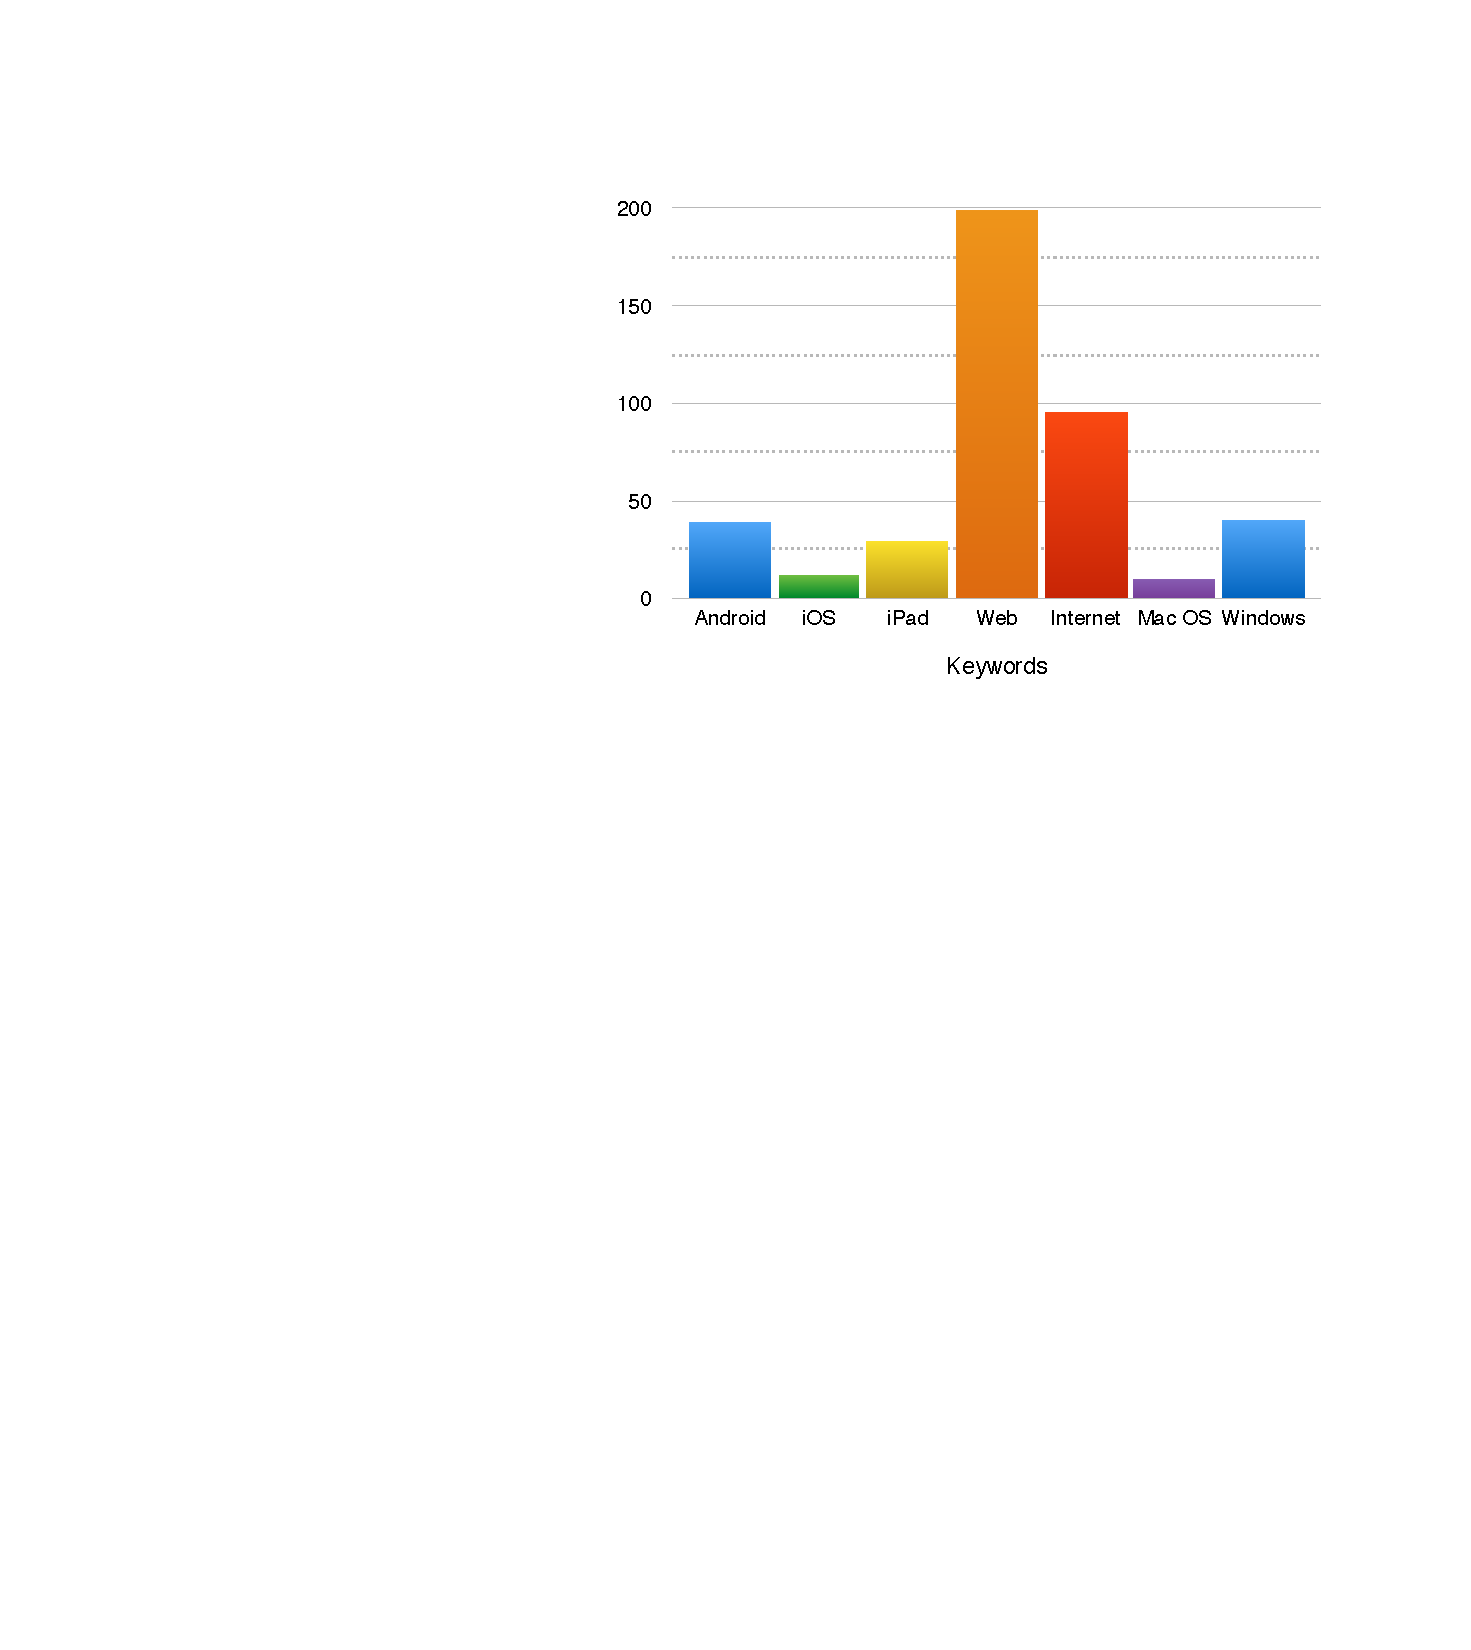
\includegraphics[width=0.90\columnwidth]{img/search}
\caption{Results of a search using Google with \emph{"music score app"} associated to different keywords. The numbers are in million hits.
\label{fig:search}}
\end{figure}

From a technical viewpoint, this change represents a move from one operating system [OS] to another. Web browsers may be viewed as a kind of OS on top of an abstract machine: they are integrating step by step all the services of an OS, up to audio services with the recent Web Audio API \cite{WebAudio}. But actually the change is far more than this simple move: 
\begin{itemize}
\item mobile platforms have adopted a fundamentaly different approach from user point of view: no traditionnal input device (keyboard, mouse), embedded sensors that may be used as controlers, a reduced graphic space especially for smartphones, a step back on multitask aspects but an wave of services composition and integration. 
\item web applications differ also due to their natural way to agglutinate distributed resources and to share content between several users. Theoretically, they can be deployed on all the platform previously mentioned.
\end{itemize}

The approach adopted by almost all music notation applications available on mobile platforms is rather classical: you can find a plethora of music score readers and players, based on the common music notation, more or less sophisticated. Music score edition is also supported by these applications but they have to re-think the user interface due to the lack of input device: handwritten recognition is one of the explored solutions\footnote{NotateMe \url{http://www.neuratron.com/notateme.html}}\footnote{StaffPad \url{http://www.staffpad.net/}}. On smartphones, the screen size limitation is not really handled, apart with messages that inform the user that the application may not be fully functional. The more innovative approaches  generally come from artistic uses \cite{polashek14a}.

On the web side, you can find online music notation editors, online score sharing systems\footnote{MuseScore \url{https://musescore.org/en/handbook/share-scores-online-0}}, or JIT compilation services like those proposed for years by the GUIDO Engine \cite{renz98}. More recently, music notation services have been made available to developers and users under the form of a RESTFUL web service \cite{solomon:2014a}. Solutions for score layout and redering can also be embedded in a web page: this is the case for the GUIDO Engine \cite{Dau:09b} that is now available as a Javascript library. 
Applications for music practising are now moving to the Internet (e.g. Weezic\footnote{\url{http://www.weezic.com/}}) but based on already existing strategies \cite{SPY05}\cite{Fober:07b}. Distributed and collaborative scores are appearing like the Flat music score editor\footnote{\url{https://flat.io/}} and also tools for network improvisation \cite{canning14a}.

Whether running on the web or on mobile platforms, the approach to music notation adopted by almost applications looks quite classical. Innovation generally comes from artistic approaches and are based on specific tools.
However, the context of mobile platforms or of the Internet could lead to new and original uses, and we think that in this regard, an adequate support is missing from tools for music notation. 

This paper proposes several use cases that are specific to the context described above.
%the Internet and to networked devices, including mobile platforms. 
These use cases may be implemented using INScore, an environment for the design of augmented interactive music scores that has been extended to support distributed scores and collaborative design, and that runs on all the major platforms (MacOS, Linux, Windows, Android and iOS). 
The paper starts with a brief reminder of the INScore environment. Next it presents the network extensions. Various use cases are then considered and a concrete realization of a dynamic score published over Internet is presented.


%-------------------------------------------------------------
\section{INScore}\label{inscore}

INScore is an environment for the design of augmented, interactive music score \cite{Fober:12a} that is entirely controled by an Open Sound Control [OSC] API \cite{Fober:12a}. It supports arbitrary graphic resources (symbolic music notation, text, images, vectorial graphics...) and displays the time relationships of the score components by the way of a simple synchronization mechanism.
INScore supports performance representation, viewed as audio or gestural signal, as well as interaction process representation also viewed as signals \cite{Fober:14b}. It includes an event based interaction mechanism \cite{Fober:13b} that provides a simple and homogeneous way to describe interactions in the graphic or the temporal space.

INScore input language is a textual version of OSC messages extended to support variables, extended OSC adresses and Javascript sections. A Javascript engine is embedded  in each score and may be remotely triggered via OSC messages.

The script below shows the example of a rectangle synchronized on a symbolic score (described using the Guido Music Notation format [GMN] \cite{hoos98}) i.e. its graphic position is computed frm it's time location. The result is illustrated in figure \ref{fig:sample1}.
\sample{
  /ITL/scene/score set gmn '[g e c a f]';\\
  /ITL/scene/rect set rect 0.05 0.3;\\
  /ITL/scene/rect color 0 0 240 120;\\
  /ITL/scene/sync rect score;\\
  /ITL/scene/rect date 3 4;
}
\begin{figure}[h]
\centering
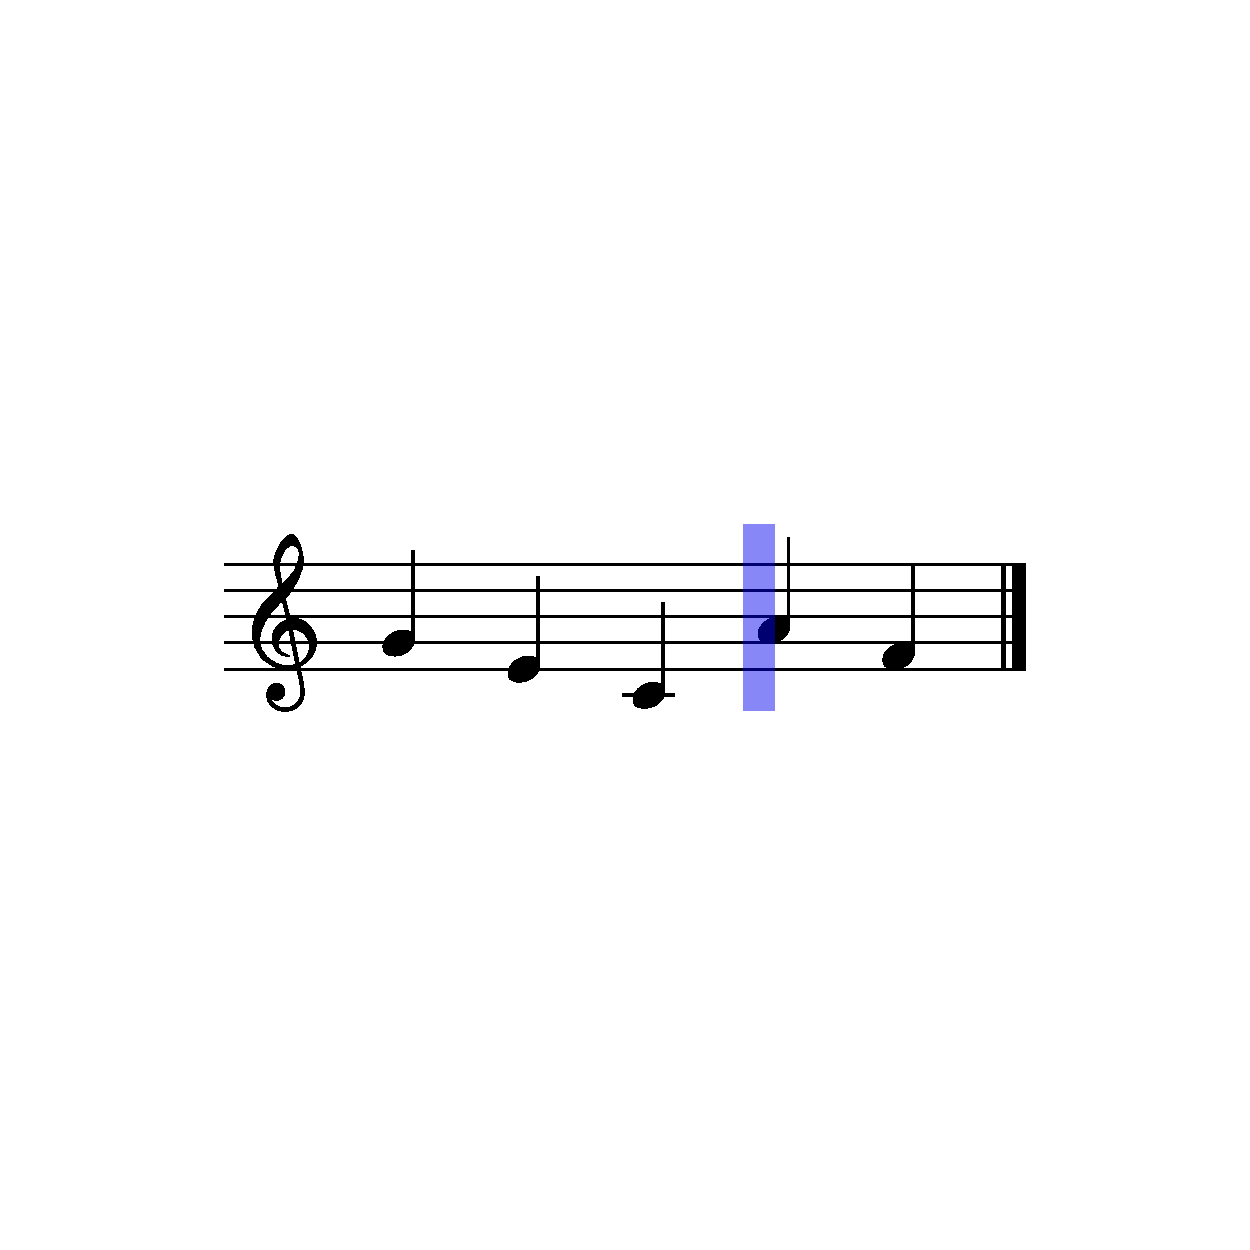
\includegraphics[width=0.60\columnwidth]{img/sample1}
\caption{A rectangle synchronized on a score.
\label{fig:sample1}}
\end{figure}

INScore has been used in many artistic projects, the last one being an implementation of Earl Brown's December Variation by Richard Hoadley \cite{hoadley14}.



%-------------------------------------------------------------
\section{INScore Web support}
INScore has been extended to support aggregation of distributed resources over Internet, as well as publication of a score via the HTTP and the WebSocket protocols.

%----------------------------------------
\subsection{Distributed score components}
Most of the components of a score can be specified in a litteral way or using a file. The example below will produce the same object, provided that the '\code{score.gmn}' file contains the \code{[g e c a f]} code.
\sample{
 /ITL/scene/score set gmn '[g e c a f]';
 \scomment{is similar to}
 /ITL/scene/score set gmnf 'score.gmn';
}

All the file based resources can be specified as a simple file path using absolute or relative path, or as an HTTP url. When using the relative path form, a file absolute path is built using the score current path, that may be set to arbitrary location using the \code{rootPath} message. This current path can be also be set to an arbitrary HTTP url, so that further use of a relative path will also result in an url.

The example below refers the same '\code{score.gmn}' file on \code{host.domain.org}.
\sample{
 /ITL/scene/score set gmnf \\
 \hspace*{6mm}      'http:://host.domain.org/score.gmn';
 \scomment{is equivalent to}
 /ITL/scene rootPath \\
 \hspace*{6mm}      'http:://host.domain.org/'; \\
 /ITL/scene/score set gmnf 'score.gmn';
}

This mechanism allows to mix local and remote resources in the same music score, but also to express local and remote scores in a similar way, using just a \code{rootPath} change.


%----------------------------------------
\subsection{HTTP and WebSocket components}

A music score can be published on the Internet using the HTTP or the WebSocket protocols. Specific components can be embedded in a music score in order to make this score available to remote clients:
\begin{itemize}
\item an HTTP server, which INScore type is \code{httpd} and  that takes a listening port number as argument,
\item a WebSocket server, which type is \code{websocket} and  that takes a listening port number and a maximum rate for clients notification as arguments.
\end{itemize}

The WebSocket server allows bi-directional communication between the server and the client. It sends notifications of score changes each time the graphic appearance of the score is modified, provided that the notification rate is lower than the maximum rate set at server creation. 

The example below creates an HTTP server that responds on the port 8000 and a WebSocket server that responds on the port 8100 and sends notifications at a maximum rate of 200 ms.
\sample{
  /ITL/scene/http set httpd 8000; \\
  /ITL/scene/ws set websocket 8100 200;
}

The communication scheme between a client and an INScore server relies on a reduced set of messages. These messages are protocol independent and can be equally supported over HTTP or WebSocket. Table \ref{tab:protocol} gives an overview of the client server communication scheme:
\begin{itemize}
\item the \code{get} message requests an image of the score. It is similar to an \code{export} message adressed to INScore, which result is sent over HTTP or WebSocket.
\item the \code{version} message requests the current version of the score. The server answers with an integer value that is increased each time the score is modified. This message is intended to allow clients to keep an up-to-date image of the score. Note that the WebSocket server automatically sends changes notifications with versionning information.
\item the \code{post} message is intended to send an INScore script to the server. The server answers with a status message which is between \code{OK} or \code{ERROR}. In case of error, details on the failure reason are provided. In case of success, the score may be modified and its current version number is increased. 
\item the \code{click} message is intended to allow remote mouse interaction with the score. The associated data should be a position in an image previously retrieved with a \code{get} message.
\end{itemize}

\begin{table}[h]
 \begin{center}
 \begin{tabular}{|l|l|l|l|}
  \hline
  Request & Data & Answer & Side effect\\
  \hline
  \code{get}  & \none & an image  & \none \\
  \code{version}  & \none & version num & \none \\
  \hline
  \code{post}  & INScore script & status & new score \\
  \code{click}  & x, y position & \none & new score \\
  \hline
 \end{tabular}
\end{center}
 \caption{INScore server Web API.}
 \label{tab:protocol}
\end{table}

%----------------------------------------
\subsection{Messages forwarding}\label{forward}

Message forwarding is another mechanism provided to distribute scores over a network. It is applied at application and score levels. It consists in a list of destination hosts specified using a host name or an IP number, and suffixed with a port number. All the OSC messages may be forwarded to the indicated hosts on the corresponding port number, provided they are not filtered out (figure \ref{fig:forward}).
The filtering strategy is based on OSC adresses and/or on INScore methods (i.e. messages adressing specific objects attributes). 

\begin{figure}[h]
\centering
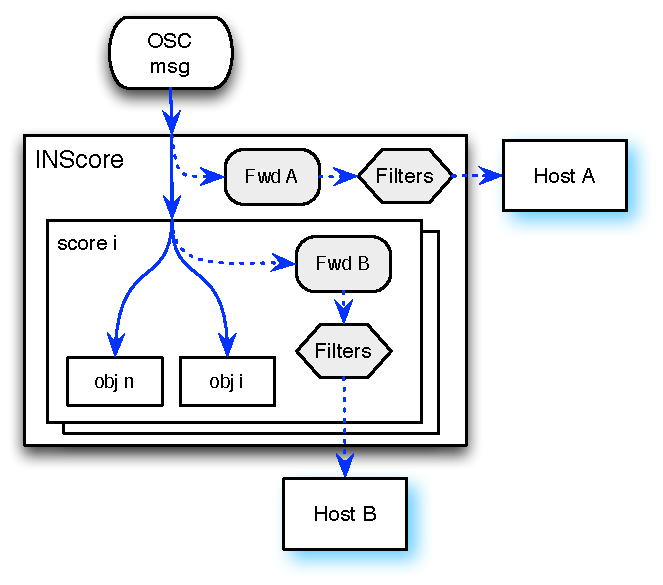
\includegraphics[width=0.90\columnwidth]{img/forward}
\caption{Message forwarding mechanism.
\label{fig:forward}}
\end{figure}

The next example installs a forwarding mechanism at application level: all the incoming messages may be forwarded to a host specified by IP number on the UDP port 7000. Next the filter is configured so that \code{clock} and \code{date} messages will not be forwarded.
\sample{
  /ITL forward 192.168.1.27:7000;\\
  /ITL/filter reject clock date; 
}


\section{Use cases}

\subsection{Groupware technologies}
Groupware technologies as described in \cite{Fober:07b} may be easily deployed using INScore and the forwarding mechanism. Let's say that we have a teacher score on a station $T$ and students on 3 stations $S1$, $S2$, $S3$.

The settings illustrated in figure \ref{fig:groupware} can be implemented with the following messages:
\begin{description}
\item A) \hspa on  T : \code{/ITL forward S1 S2 S3;}
\item B) \hspa on  T : \code{/ITL forward S1;}\\
on  S1 : \code{/ITL forward T;}
\item C) \hspa on  T : \code{/ITL forward S1 S2 S3;}\\
on  S1 : \code{/ITL forward T;}
\end{description}

\begin{figure}[h]
\centering
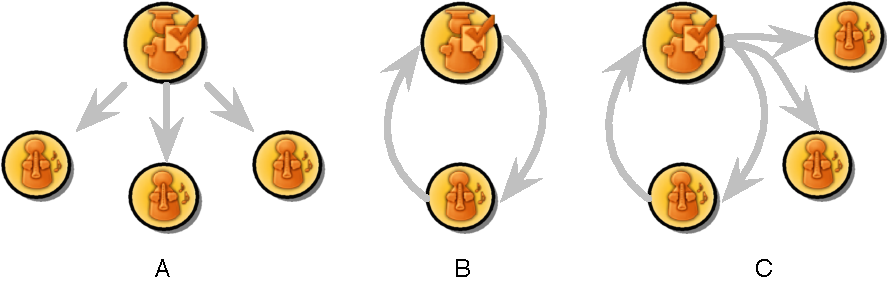
\includegraphics[width=0.95\columnwidth]{img/groupware}
\caption{Use cases in a pedagogic setting: A)the teacher score is published to the students, B) the teacher and the student interact with the same score, C) the setting is similar to B) but the score is published to the other students that can look at the interaction.}
\label{fig:groupware}
\end{figure}


\subsection{Collaborative score design}

Collaborative score design could be implemented with any number of participants, i.e. all the participants can interact with a score that is available to all the others, also in read/write mode. We assume that one station is the central point of messages distribution, then the forwarding scheme illustrated in figure \ref{fig:collabscore} is describe below:
\sample{
on A: /ITL forward B C;\\
on B: /ITL forward A;\\
on C: /ITL forward A;
}

\begin{figure}[h]
\centering
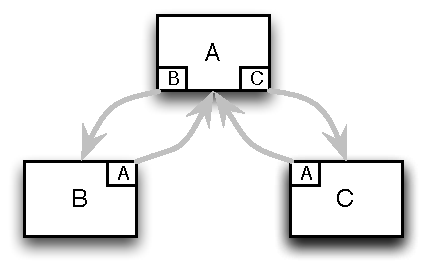
\includegraphics[width=0.5\columnwidth]{img/collabscore}
\caption{Collaborative score design.}
\label{fig:collabscore}
\end{figure}

Note that the forwarding scheme could be setup from the same computer using INScore extended OSC addresses (e.g. \code{B:/ITL/forward A})

Note also that the forwarding mechanism prevents messages to be forwarded to the sender and thus, avoids direct loops (but not indirect loops e.g. A $\to$ B $\to$ C $\to$ A).


\subsection{Shared score over Internet}

Although the forwarding scheme above is basically intended to run on a local network, it could be implemented over the Internet as well, but since the underlying communication protocol is UDP, it may face significant packets losses, depending on the network conditions.

A secure solution to collaborative design may use the HTTP or WebSocket servers. The example below implements a score that displays the local score and includes a remote score as illustrated in figure \ref{fig:sharedscore}.

\begin{figure}[h]
\centering
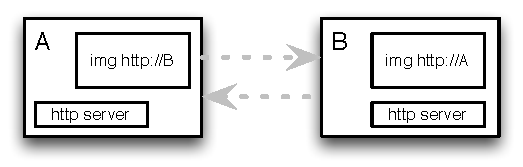
\includegraphics[width=0.8\columnwidth]{img/sharedscore}
\caption{Scores shared over the Internet.}
\label{fig:sharedscore}
\end{figure}

\sample {
	On each station: \\
\hspace*{5mm}	/ITL/scene/http set httpd 8000;
\hspace*{5mm}	/ITL/scene/remote set img \\
	\hspace*{25mm}'http://remote.address';
}

Note that using a \code{websocket} object instead of \code{httpd} could make the remote view refreshment transparent. To do so, the \code{ws://} protocol has to be implemented for file based resources. That's one of the future directions.


\subsection{Audience score based interaction}
The INScore internet protocols support UI interactions and notably, relay the user clicks or touch screen interactions to the server. It is thus easy to imagine a concert setting where the music score is published (e.g. using the \code{websocket} server) and where the audience could get the score on a mobile phone and interact with it in real-time using the event based interaction mechanism of INScore, modifying the course of the music piece. 


\subsection{Flux Aeterna}

\textit{Flux \AE terna} has been composed by Vincent Carinola in 2014. The piece has been designed for the Internet\footnote{\url{http://vr.carinola.free.fr/fluxaeterna/}}. It comes under the form of an endless audio stream. The listening conditions are similar to those of a web radio but here, the listener can  influence the future of the piece by providing its own sound files.

A dynamic score of the piece has been designed using INScore. The piece is using Max/MSP that sends modules and events information to INScore in real-time via OSC. This information is converted into a graphic information that reflects the piece structure (figure \ref{fig:flux}) using the embedded Javascript engine. 

\begin{figure}[h]
\centering
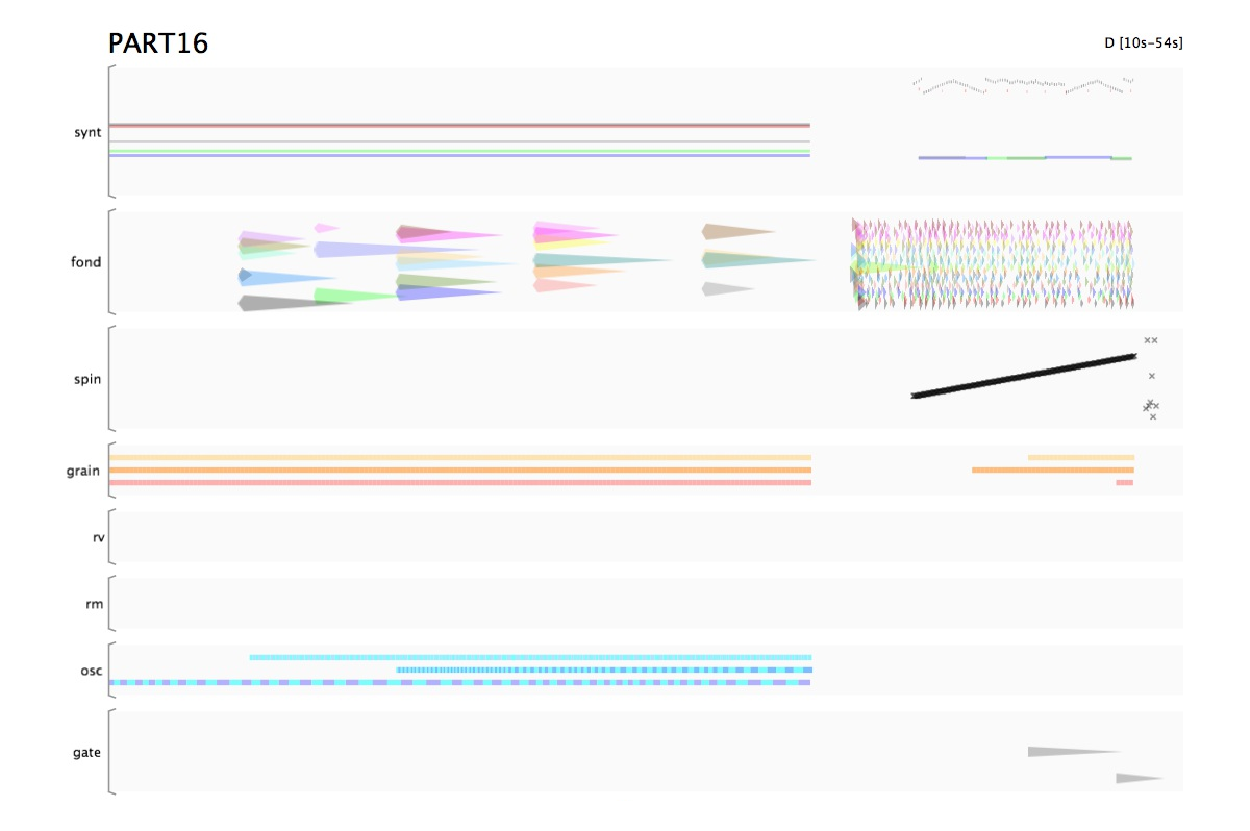
\includegraphics[width=0.95\columnwidth]{img/flux}
\caption{One page of Flux \AE terna.}
\label{fig:flux}
\end{figure}

The score has been initially designed for a local display, in the context of an exhibition. Adding a simple \code{httpd} or \code{websocket} object to the score allows to make it public over Internet, as illustrated with the HTTP example below:
\sample{
/ITL/scene/server set httpd 8000;
 \scomment{makes the score available at}
http://thehost.thedomain.org:8000
}

In addition, the score may be distributed in real-time to any INScore viewer connected to the local network using the forwarding mechanism mentionned in section \ref{forward}. The script below forwards the messages to any INScoreViewer running on a device connected to the local network. Messages addressed to the Javascript engine are filtered in order to only forward the result of their evaluation.
\sample{
/ITL forward 192.168.1.255;\\
/ITL/filter reject '/ITL/scene/javascript';
}


\section{Conclusions}

Applications for music notation are moving to mobile platforms and to the web, following the general stream of  computing migration. Most of these applications are reproducing the existing approaches to music notation although their deployment on the web and/or mobile platforms could take advantage of the technological context to create innovative uses. Actually, innovation exists but it is restricted to specific applications, mostly designed in artistic projects. With its network extensions and its support for Android and iOS, INScore provides a set of solutions for distributed score design and interaction. The approach tends to make network support as transparent as possible in a score description. Future extensions should make remote resources available using the \code{WebSocket} protocol, which should ma-ke remote files refreshment transparent and allow additional use cases in the domain of shared and collaborative score design.



\begin{acknowledgments}
INScore research and development has been funded by the French National Research Agency [ANR].\\
INScore is an open source project hosted on SourceForge {\small (\url{http://inscore.sf.net})}
\end{acknowledgments} 

%%%%%%%%%%%%%%%%%%%%%%%%%%%%%%%%%%%%%%%%%%%%%%%%%%%%%%%%%%%%%%%%%%%%%%%%%%%%%
%bibliography here
\balance
\bibliography{../interlude}

\end{document}
